\section{Finaler Entwurf}
\subsection{Entwurfsziele}
Im finalen dritten Entwurf sollen nun diese Überlegungen realisiert werden, um den Beschleuniger endlich auf die erforderliche Größe
zu bringen. Konkret soll der Datenspeicher in den BRAM verschoben werden. Dazu sollen zwei BRAM-Einheiten verwendet werden, auf die
die Recheneinheiten über zwei Kanäle zugreifen können. Zusätzlich soll die Berechnung der $\rho$-Funktion über ein Schieberegister so realisiert werden,
dass sie ihre Daten aus dem BRAM lesen und schreiben kann. Da der BRAM mit Tiles arbeitet, muss außerdem das Einlesen der Datenblöcke,
sowie das Ausgeben des Endergebnisses über eigene Komponenten gesteuert werden, die den Datenaustausch zwischen der Kommunikationsschnittstelle
und dem BRAM übernehmen. Durch den Einsatz des BRAM entsteht jedoch noch ein Problem: Die Eingabedaten liegen im Hauptspeicher Lane-orientiert vor.
Um sie in den BRAM schreiben zu können, müssen sie in Tiles umgeordnet werden. Dieser Prozess muss entweder vor der Berechnung mühsam in Software
ausgeführt werden, oder die Konvertierung findet im Beschleuniger selber statt. Die Konvertierung in Software würde viel extra Rechenzeit in Anspruch
nehmen. Deshalb werden wir sie im Beschleuniger durchführen. Da aber noch nicht klar ist, wie viel Platz in den Atomen nach den Änderungen vorhanden sein wird,
wird die Konvertierung in zwei weiteren Atomen parallel zur Berechnung der KECCAK-p-Funktion durchgeführt.

\subsection{Aufbau}
\begin{figure}
	\center
	\includegraphics{images/iteration_3.pdf}
	\caption{Aufbau der A-Atome}
	\label{fig:aufbau_iteration_3}
\end{figure}
\begin{figure}
	\center
    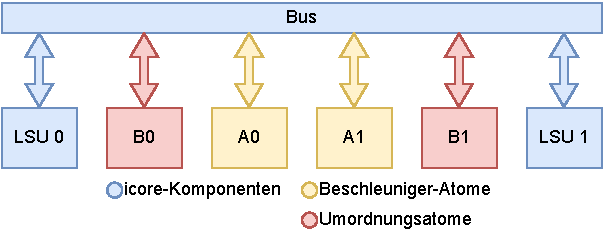
\includegraphics{images/Iteration_3_Integration.pdf}
	\caption{Integration der Atome im finalen Beschleuniger}
    Unbenutzte Komponenten und Kontrollsignale wurden weggelassen
	\label{fig:iteration_3_integration}
\end{figure}
\begin{figure}
	\center
	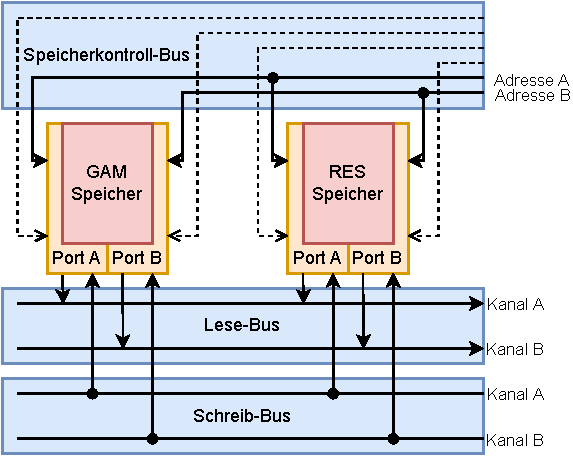
\includegraphics{images/Speicheranbindung.pdf}
	\caption{Speicheranbindung}
	\label{fig:speicheranbindung_iteration_3}
\end{figure}
Der Beschleuniger besteht diesmal aus insgesamt vier Atomen. Die beiden Atome \textit{A0} und \textit{A1} sind wie ihre Vorgänger symmetrisch und
sind für die eigentliche Berechnung der Permutationsfunktion zuständig (siehe Abb. \ref{fig:aufbau_iteration_3}). Die Atome \textit{B0} und \textit{B1} lesen während der Berechnung schon
den nächsten Datenblock aus dem externen Speicher ein und konvertieren ihn in Tiles, die dann von den A-Atomen entgegen genommen werden.
Wie auch im vorherigen Entwurf wird den Atomen ihre Rolle über einen Atom-Index zugewiesen. In Abbildung \ref{fig:iteration_3_integration}
ist dargestellt, wie die Atome in der Fabric des i-Core angeordnet sind. Die Funktionalitäten der A-Atome "Daten lesen", "Ergebnis schreiben",
"$\rho$ berechnen" und "$\gamma$ berechnen" haben ihre eigenen Berechnungseinheiten erhalten. Verbunden sind alle Komponenten über eine Infrastruktur
aus Bussen und einem Kommunikationsmodul für den Datenaustausch mit anderen Atomen. Verwaltet wird die gesamte Berechnung wieder von einem Zustandsautomaten.

\subsubsection{BRAM}
Die beiden verwendeten BRAM-Bänke GAM (für Gamma) und RES (für Result) besitzen jeweils zwei Lese-Schreib-Ports, mit denen jeweils zwei Tiles
gelesen und auch gleichzeitig geschrieben werden kann (read before write). Je ein Port ist dabei an den A-Kanal und der Andere an den B-Kanal angeschlossen,
sodass insgesamt bis zu vier Tiles gleichzeitig gelesen und geschrieben werden können. 

\subsubsection{Speicherbus}
Der Speicherbus besteht aus drei Segmenten (Abb. \ref{fig:speicheranbindung_iteration_3}). Auf dem Lese-Bus werden Daten aus dem BRAM ausgelesen und den anderen Modulen zur Verfügung gestellt.
Er besteht aus zwei Kanälen, die beide zwei Tiles breit sind.
Auf dem Schreib-Bus werden Daten von den Berechnungsmodulen und dem Kommunikationsmodul gesammelt und an den BRAM weitergegeben.
Er ist auch zwei Tiles breit. Über den Speicherkontroll-Bus werden alle Steuersignale für den BRAM gesammelt.
Er besteht aus zwei 7 Bit breiten Adress-Vektoren für die beiden Datenkanäle, sowie einem Read-Enable-Signal
und einem Write-Enable-Signal für jeden der insgesamt vier Ports.

\subsubsection{Zustandsautomat}
Der Zustandsautomat besteht nicht mehr aus einer Einheit, sondern besteht nun aus einer zentralen Kontrolle, dem Manager,
sowie spezialisierten Kontrolleinheiten innerhalb der Berechnungseinheiten, angedeutet durch die kleinen lila Blöcke oberhalb der Berechnungseinheiten.
Der Manager steuert dabei nur noch den Betriebsmodus des Kommunikationsmoduls und stößt die Abarbeitung in den Berechnungseinheiten an.
Die Zustandskontrolle innerhalb einer Berechnungseinheit bekommt bei Aktivierung die Kontrolle über den Speicherkontroll-Bus
und generiert die Steuersignale für die Berechnungseinheit und den Speicher. Ist die Abarbeitung einer Berechnungseinheit abgeschlossen,
wird die Kontrolle über den Speicher und die weitere Abarbeitung wieder an den Manager übergeben.

\subsubsection{Kommunikationsmodul}
Das Kommunikationsmodul dient zum Datenaustausch zwischen den Atomen sowie zur Kommunikation mit dem externen Speicher, der die Eingabedaten bereitstellt und das Ergebnis entgegennimmt.
Für jede Berechnungseinheit gibt es einen Betriebsmodus, der festlegt, welche Daten von der Berechnungseinheit und dem Speicherbus ausgegeben werden und welche empfangenen Daten
an den Speicherbus und die Berechnungseinheit weitergegeben werden. Dieser Betriebsmodus wird vom Manager bestimmt.

\subsubsection{Gamma}
Das Gamma-Modul berechnet analog zum Modul aus dem vorherigen Entwurf immer zwei Slices und gibt die entsprechenden Tiles
an den Speicher und über das Kommunikationsmodul an das andere Atom aus. Bis auf die Einführung des Kontrollblocks
und einer leichten Anpassung der Schnittstelle ist es identisch zum vorherigen Design.
Es nimmt die Eingabedaten vom RES-Speicher und dem Kommunikationsmodul entgegen und schreibt das Ergebnis der Berechnung in den GAM-Speicher,
bzw. übermittelt es die restlichen Tiles wieder über die Kommunikationseinheit an das andere Atom, wo sie gespeichert werden.

\subsubsection{Rho-Puffer}
\begin{figure}
	\center
	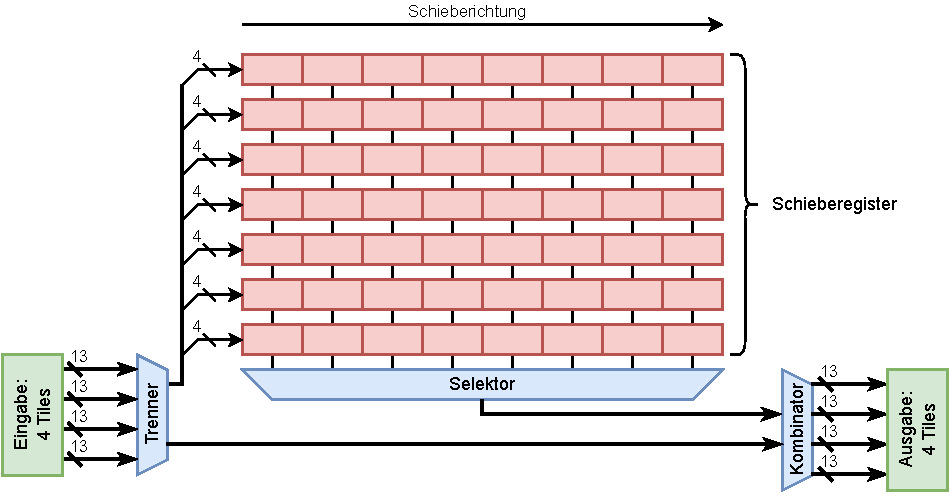
\includegraphics{images/Rho-Aufbau.pdf}
	\caption{Aufbau des Rho-Puffers}
	\label{fig:rho_aufbau_iteration_3}
\end{figure}
Der Rho-Puffer besteht aus sieben 32-Bit-Schieberegistern. Diese berechnen, wie in \ref{cha:iteration_2_rho_transformation} beschrieben,
interativ die Rotationen der $\rho$-Funktion. Der Aufbau des Rho-Moduls ist in Abbildung \ref{fig:rho_aufbau_iteration_3} skizziert.
Die Berechnung erfolgt wie folgt: Im ersten Schritt werden die Tiles aus dem GAM-Speicher gelesen und auf den betreffenden Lanes
wird eine Linksrotation durchgeführt, während die anderen Lanes unverändert bleiben. Das Ergebnis wird im wieder im GAM-Speicher gespeichert.
Im zweiten Schritt werden die Tiles aus dem GAM-Speicher erneut ausgelesen und diesmal wird auf den übrigen Lanes eine Rechtsrotation durchgeführt.
Das finale Ergebnis der $\rho$-Berechnung wird dann im RES-Speicher wieder abgespeichert. Da es zur Berechnung keinerlei Kommunikation benötigt,
ist dieses Modul auch als einziges nicht an die Kommunikationseinheit angeschlossen.

\subsubsection{Einlesemodul}
Um das Ergebnis einer Permutation mit einem neuen Datenblock gemäß der Schwammkonstruktion zu kombinieren, müssen die eingelesenen Daten
mit den Daten im Ergebnisspeicher mit einem XOR kombiniert werden. Das Einlesemodul macht genau das und schreibt die kombinierten Daten
wieder zurück in den Ergebnisspeicher, sodass erneut die Permutation berechnet werden kann. Während die neuen Daten eingelesen werden,
kann jedoch die eigentliche Berechnung nicht durchgeführt werden. Daher ist es wichtig, dass dieser Schritt so schnell wie möglich abläuft.
Dazu werden die Daten den A-Atomen beim Einlesen direkt als Tiles bereitgestellt, sodass das Einlesemodul nicht erst die Lanes in Tiles konvertieren muss.
Diese Aufgabe übernehmen, wie bereits beschrieben, die B-Atome.

\subsubsection{Ergebnismodul}
Zur Ausgabe des 256-Bit Hashes wird das Ergebnismodul verwendet. Es besteht aus einem in Flip-Flops implementierten Puffer,
der mit den Daten des Ergebnisspeichers gefüllt wird und die Daten so zurück in Lanes konvertiert.
So kann das Ergebnis direkt im richtigen Format ausgegeben werden und im externen Speicher übernommen werden.

\subsection{Berechnung der Permutationsfunktion}
Da die Daten im BRAM nur als Tiles gespeichert werden und die Eingabedaten aber als Lanes vorliegen, müssen sie erst konvertiert werden.
Diese Konvertierung findet während der vorherigen Berechnung in den B-Atomen statt.
Dabei lesen die B-Atome mehrfach den gesamten Datenblock Lane für Lane ein und puffern immer einen Teil aller Lanes, bis sie sie als vollständige Tiles speichern können.
Dass dabei jede Lane mehrfach eingelesen werden muss, hat keinen Einfluss auf die Ausführungszeit des Beschleunigers, da die Berechnungszeit der modifizierten Rundenfunktion größer ist,
als die Berechnungszeit der Konvertierer und beide Systeme vollständig parallel arbeiten können.
Nachdem ein Block konvertiert wurde und die A-Atome bereit sind, werden die Tiles der Reihe nach über das Kommunikationsmodul von den B-Atomen zum Einlesemodul der A-Atome übertragen
und mit den Daten aus dem RES-Block über ein XOR kombiniert und anschließend wieder in den RES-Block übernommen.
Für die Gamma-Berechnung werden die Slices über den Lesebus aus dem RES-Block gelesen und an die Recheneinheit sowie an die Kommunikationseiheit übergeben.
Die Ergebnisse werden anschließend vom Kommunikationsmodul und der Recheneinheit über den Schreib-Bus in den GAM-Block geschrieben.
Anschließend wird die Links-Rotation mit Hilfe des Rho-Puffers durchgeführt. Die Daten werden aus dem GAM-Block über den Datenbus an den Puffer übertragen.
Zuerst wird der Puffer mit den Initialdaten gefüllt, dann werden, wie in \ref{cha:iteration_2_rho_transformation} erläutert, die Tiles nach und nach in den Puffer eingeschoben
und die Ergebnis-Tiles werden über den Schreib-Bus wieder in den GAM-Block übernommen.
Die Rechts-Rotation wird analog durchgeführt, nur werden dieses Mal die Ergebnisse in den RES-Block geschrieben anstatt in den GAM-Block.
Hier wird auch ein Vorteil des Bus-Designs deutlich: Da beide Blöcke ihre Daten über den Bus empfangen, braucht für die Rechts-Rotation nur das
Write-Enable-Signal verändert werden und die Ergebnisse müssen nicht auf eine andere Eingabe umgeleitet werden.
Die Rho und Gamma Funktionen werden so oft abwechselnd berechnet, bis der Datenblock gemäß der Definition der KECCAK-p-Funktion verarbeitet wurde.
Danach kann über den Kontrollvektor von außen bestimmt werden, ob entweder der nächste Block eingelesen werden, oder das Ergebnis ausgegeben werden soll.
Für die Ausgabe des Ergebnisses werden alle 64 Tiles im Atom A0 vom Ergebnismodul ausgelesen und die ersten 4 Bits im Puffer des Ausgabemoduls gespeichert.
Als letztes wird das Ergebnis als Lanes ausgegeben und im externen Speicher als Endergebnis gespeichert.

\subsection{Bewertung}
Die A-Atome erfüllen mit einer Größe von 1205 LUTs die Anforderungen des i-Core, was das Hauptziel dieses Entwurfs war.
Leider wurde dafür sehr viel Berechnungsgeschwindigkeit geopfert. Mit weiteren Optimierungen lässt sich der noch verfügbare Platz
bestimmt sinnvoll nutzen, um die Berechnung wieder etwas zu beschleunigen. Wie solche Ansätze aussehen könnten, werden wir uns später
ansehen. Außerdem besteht der Beschleuniger jetzt aus vier Atomen. Die B-Atome sind dabei sehr unspektakulär, weshalb wir sie uns auch
nicht weiter angeschaut haben. Sie sind mehr eine Bequemlichkeitslösung, um sich nicht mit der Integration des Konvertierungsprozesses
in die A-Atome beschäftigen zu müssen, als dass sie sonderlich hilfreich bei der Berechnung sind. Weitere Optimierungsansätze sollten
sich daher vor allem darauf fokussieren, diese B-Atome entweder loszuwerden, oder sinnvoll für die Berechnung zu nutzen.
Was jedoch sehr schön funktioniert, ist die Berechnung der modifizierten Rundenfunktion in den einzelnen Modulen.
Ohne die Berechnung der $\rho$-Funktion über die Schieberegister wäre dieses Verfahren nicht möglich gewesen.
Die Frage, wie gut der Beschleuniger die Berechnung von KECCAK-p und damit auch SHA-3 denn jetzt tatsächlich beschleunigt,
werden wir uns im nächsten Kapitel anschauen.